%--------------------------------------------------------------------------------------
% Dokumentum formátuma [Document format]
%--------------------------------------------------------------------------------------
\documentclass[12pt,a4paper,oneside]{article}

%--------------------------------------------------------------------------------------
% Csomagok inicializálása [Initializing packages]
%--------------------------------------------------------------------------------------

\usepackage[utf8]{inputenc}
\usepackage[magyar]{babel}
\usepackage{t1enc}
\usepackage{amsmath}
\usepackage{amsfonts}
\usepackage{amssymb}
\usepackage{geometry}
\geometry{
    top=20mm,
    bottom=20mm,
    left=20mm,
    right=20mm,
}
\usepackage{hyperref}
\usepackage{mathrsfs}
\usepackage{fancyhdr}
\usepackage{graphicx}
\usepackage{icomma}
\usepackage{adjustbox}
\usepackage{lastpage}
\usepackage{float}
\usepackage{pdfpages}
\usepackage{subcaption}
\usepackage{tocloft}
\usepackage{bm}
\usepackage{multicol}
\usepackage{listings}
\usepackage{tikz}
\usepackage[abs]{overpic}
\usepackage{pict2e}

%--------------------------------------------------------------------------------------
% Dokumentum törzse [Document body]
%--------------------------------------------------------------------------------------

\begin{document}

%--------------------------------------------------------------------------------------
% Címoldal [Titlepage]
%--------------------------------------------------------------------------------------

\author{\textit{Készítették:}\\ Buczny Dominik \hspace{5pt} Hanich Péter \\ Németh Gergő Olivér \hspace{5pt} Olchváry Ambrus \\[10pt] \textit{Konzulens:}\\ Gazdi László}
\title{Szoftverarchitektúrák Házi Feladat \\ Író-olvasó oldal \\ \textbf{Specifikáció}}
\date{2024/2025/1}
\maketitle
\thispagestyle{empty}
\begin{center}
    
\includegraphics[width=\textwidth,height=\textheight,keepaspectratio]{./figures/logo.png}
\end{center}  

%--------------------------------------------------------------------------------------
% Tartalomjegyzék [Table of Contents]
%--------------------------------------------------------------------------------------
\newpage
\tableofcontents
\thispagestyle{empty}
\newpage

%--------------------------------------------------------------------------------------
% Oldalszámok formázása [Page numbering]
%--------------------------------------------------------------------------------------
\fancyhf{}
\lhead{Szoftverarchitektúrák}
\rhead{VIAUMA21}
\cfoot{\thepage}
\pagestyle{fancy}
\setcounter{page}{1}


%--------------------------------------------------------------------------------------
% Tartalom [Contents]
%--------------------------------------------------------------------------------------

%TODO A tartalmat ide írd  [Write the chapters here]
% Ki lehet file-okba is szervezni [You can organize it into files]
% Példa: \include{sections/introduction}

\section{A rendszer célja, funkciói, környezete.}

\subsection{Feladatkiírás}
A feladat egy író-olvasó oldal elkészítése. Az oldalon a regisztrált felhasználók olvashatják egymás megosztott történeteit, azokhoz megjegyzéseket, kritikákat fűzhetnek. A történeteket legyen lehetőség gyűjteményekbe, a fejezeteket regényekbe szervezni. A feltöltött történetek minden esetben moderátori ellenőrzésen esnek át, csak ez után érhetőek el publikusan. A moderálás eredményéről a felhasználót mindenképpen értesíteni kell. A történeteket el lehet látni jellemzőkkel, illetve meg lehet jelölni a kategóriájukat, a benne szereplő karaktereket, valamint figyelmeztetéseket és korhatárt lehet rájuk beállítani. Ezen kívül a regisztrált felhasználóknak lehetőségük van egymással privát üzenetben kommunikálni. A rendszerhez webes és mobilos kliens készítése is szükséges.
A részletes követelmények a \textit{Specifikáció} dokumentumban találhatók.
Mi a feladatkiírástól némileg eltérő nevezéktant használtunk: a továbbiekban a \textit{történet} helyett a \textit{mű} szót használjuk.

\subsection{A rendszer által biztosított funkciók}

A specifikáció alapján a platform a következő főbb funkciókat hivatott biztosítani. 
(Az egyes funkciók különböző szintű jogosultságokhoz kötöttek lehetnek.):
\begin{itemize}
    \item  Regisztráció
    \item  Bejelentkezés
    \item  Művekkel kapcsolatos funkciók:
    \begin{itemize}
        \item Történetek böngészése
        \item Történetek keresése
        \item Történetek olvasása
        \item Történetek létrehozása
        \item Történetek szerkesztése, fejezetekre osztása
        \item Történetek moderálása

    \end{itemize}
    \item  Gyűjteményekkel kapcsolatos funkciók:
    \begin{itemize}
        \item Gyűjtemények böngészése
        \item Gyűjtemények keresése
        \item Gyűjtemények megtekintése
        \item Gyűjtemények létrehozása 
    \end{itemize}
    \item  Hozzászólás írása Művekhez vgy Gyűjteményekhez
    \item  Művek, Gyűjtemények, Hozzászólások kedvelése
    \item  Privát üzenetek küldése
\end{itemize}

A rendszer az alábbi szerepköröket különbözteti meg: látogató, regisztrált felhasználó, moderátor, adminisztrátor. 
A látogatók csak a megosztott tartalmakat tekinthetik meg, a regisztrált felhasználók létrehozhatnak saját tartalmat, kommentelhetnek, kedvelhetnek és üzeneteket küldhetnek.
A moderátorok a moderálási jogosultságokkal rendelkeznek, az adminisztrátorok pedig a teljes rendszer felett rendelkeznek, kezelik a jogosultságokat.

\subsection{A rendszer környezete}

--- Backend és web környezetének leírása ---

A mobil kliens platformspecifikus, android operációs rendszerre készült kotlin nyelven Android Studioban.
A felhasználói felület normál méretű mobiltelefonra lett optimalizálva, egyéb méretű eszközökön (pl. okosórán) nem lett tesztelve.
A mobil kliens használatához internetelérés szükséges, az alkalmazás elérje  a backend szolgáltatásokat. 

\section{Megvalósítás}
\label{sec:implementation}


A szoftver három fő komponensből áll össze: a backend, a webes kliens és a mobil kliens.
A hárokomponens klasszikus kliens-szerver architektúrát valósít meg: a backend a szerveroldali logikát, a webes és a mobilos kliens 
felhasználói felületet.
A backend és a kliensek közötti kommunikáció http protokollon keresztül történik, a backend REST API-t biztosít a kliensek számára.
Az egyes komponensek fejlesztését, külön külön végeztük, így a fejlesztőcsapat tagjainak jól elkülönülő feladata és felelősségi körük volt.
\subsection{Architektúra}

A szoftver egészében és komponenseiben is rétzegzett architektúrát valósít meg, melynek egy áttekintő ábrája látható a \ref{fig:architecture} ábrán.

\begin{figure}[H]
    \centering
    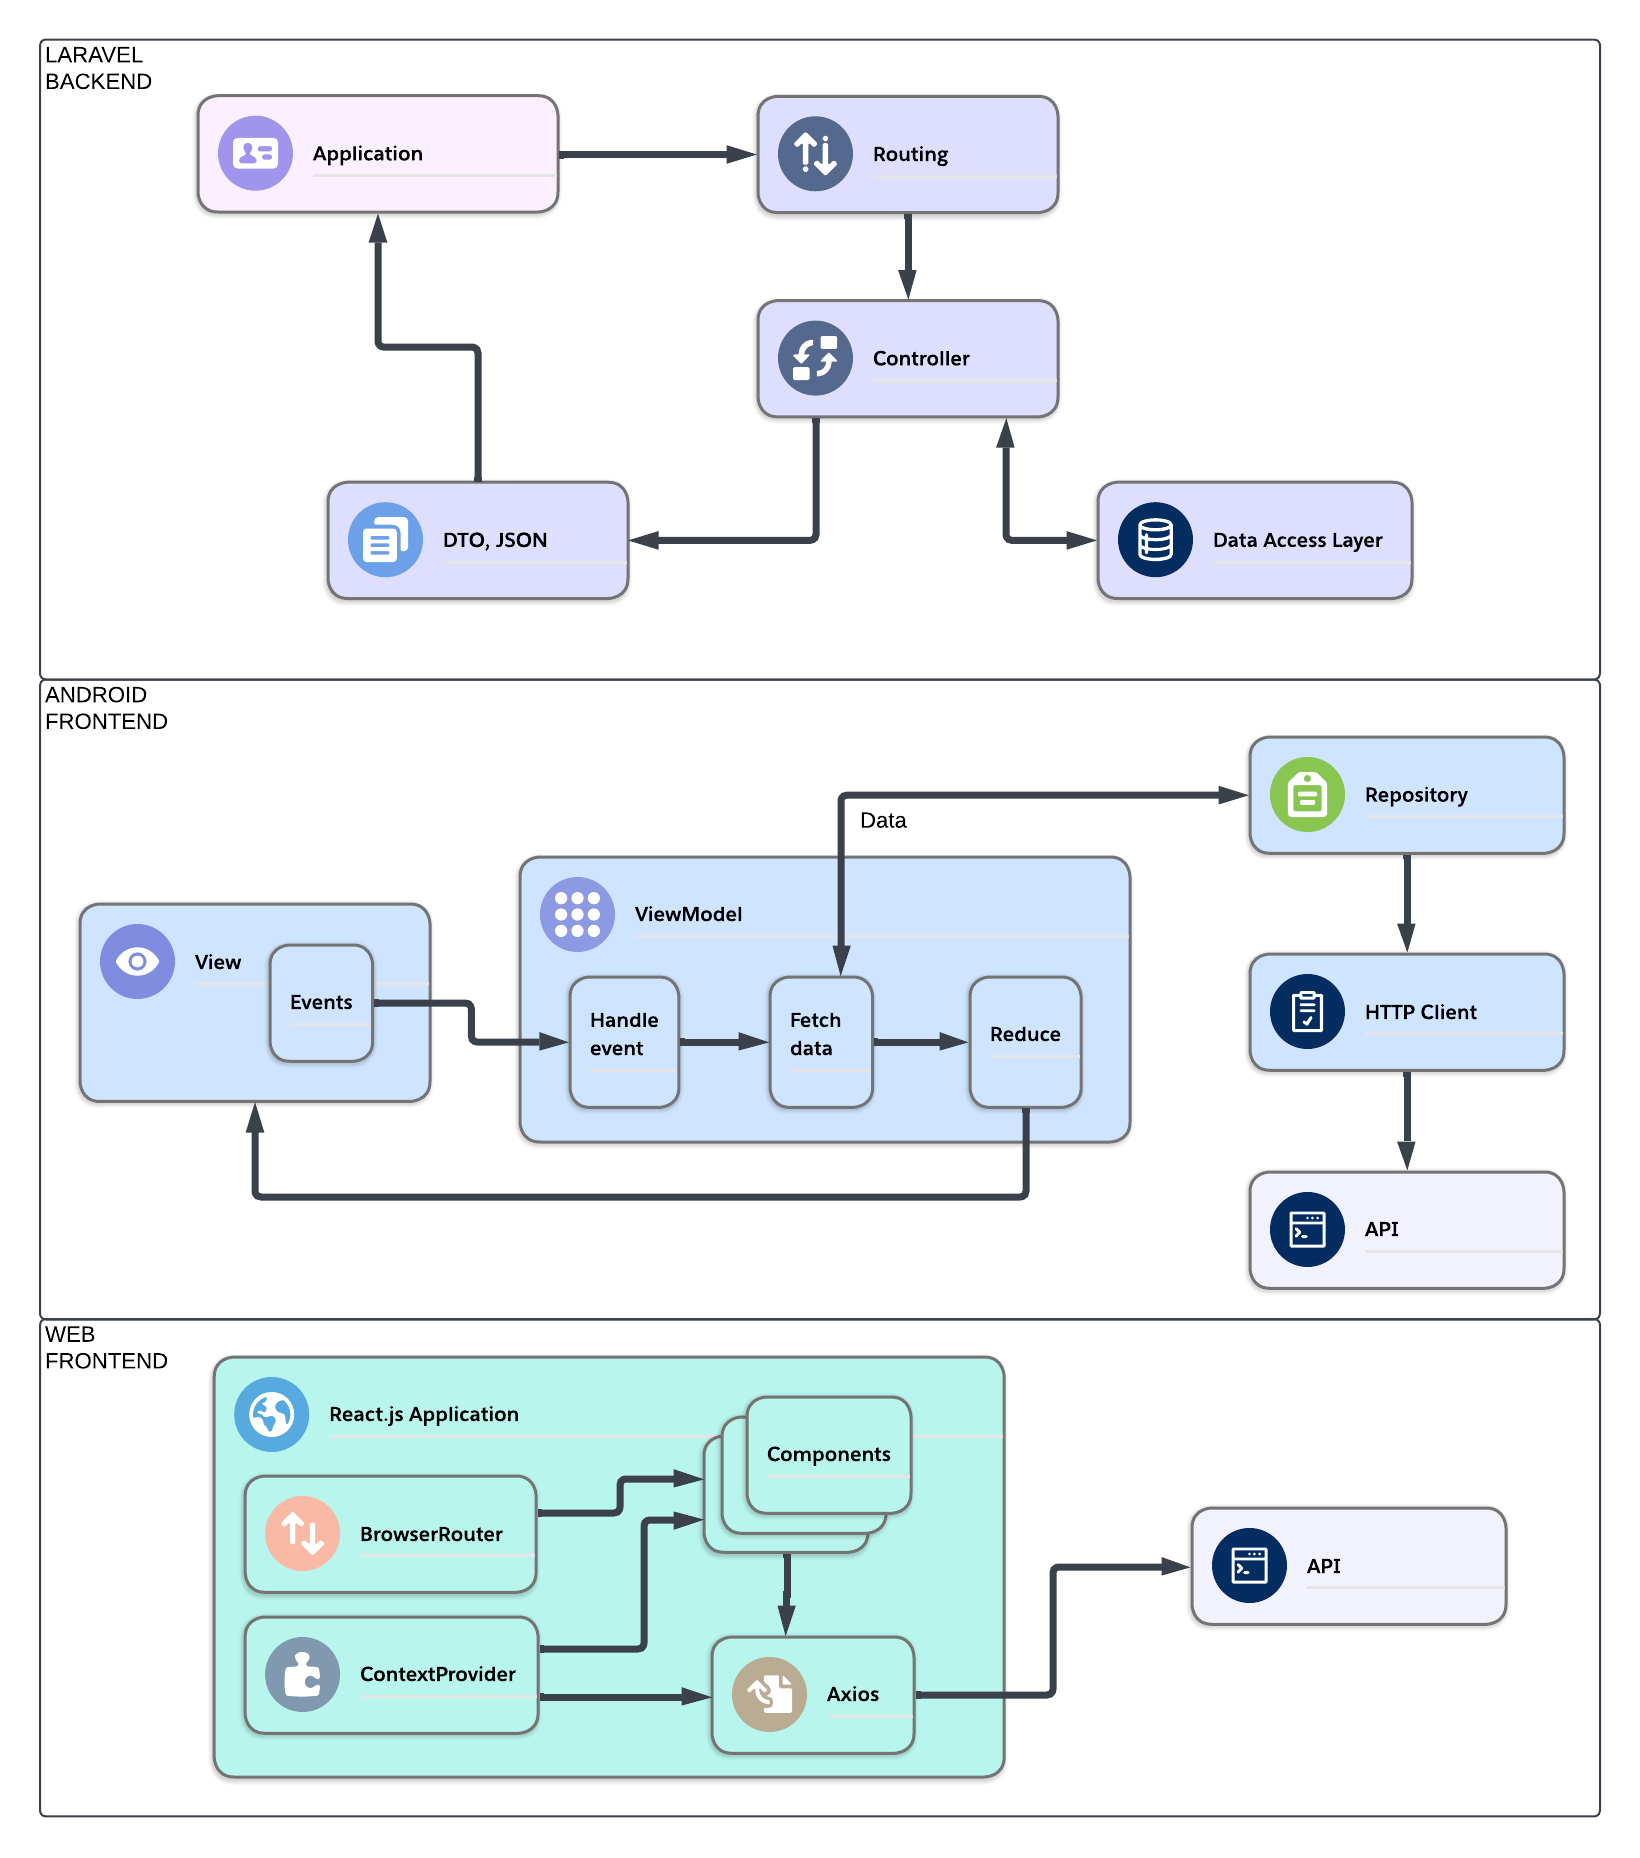
\includegraphics[scale=0.5]{./figures/architecture.png}
    \caption{A szoftver architektúrája}
    \label{fig:architecture}
\end{figure}

A szoftver egy kliens-szerver architektúrát valósít meg, ahol a kliensek a szerverrel REST API-n keresztül kommunikálnak. A szerver oldali alkalmazás a Laravel PHP keretrendszer segítségével készült, míg a kliens oldali alkalmazás két részre osztható: egy webes frontendre, mely a React keretrendszerre épül, és egy mobil kliensre, mely a JetPack Compose keretrendszer segítségével készült.

\subsubsection{Backend architektúra}

A Laravel alapból az MVC (Model-View-Controller) architektúrát követi, azonban a projektünkben a nézeteket a kliensek kezelik, így csak a Modell és a Controller rétegek maradnak meg. Így a Laravel alkalmazásunk 2 fő rétegre osztható:

\begin{itemize}
    \item Adathozzáférési réteg (Data Access Layer)
    \item Üzleti logikai réteg (Business Logic Layer)
\end{itemize}

A kliensekkel való kommunikáció REST API-n keresztül történik, így a Laravel alkalmazásunkban a REST API végpontok implementációja a kontrollerekben található. A küldött és fogadott adatok JSON formátumban vannak, melyek a Laravel által biztosított Resource osztályok segítségével könnyen kezelhetőek, melyek egyfajta DTO (Data Transfer Object) mintaként működnek.

\subsubsection{Mobilos kliens}

A mobilos kliens 2 fő rétegre osztható:

\begin{itemize}
    \item  [1.] Adat réteg (Data Layer)
    \begin{itemize}
        \item Adatlekérdezési réteg (HTTP kliens): REST API hívások implementációja, JSON objektumok kotlin osztályokra való leképezése.
        \item Adatelérési réteg (Repository): hálózati kommunikáció és hibakezelés és egységesített kezelése, magasabb szintű kódban könnyebben használható.
    \end{itemize}
    \item  [2.] UI réteg (UI Layer)
    \begin{itemize}
        \item  Állapotkezelés (View Model)
        \item  Megjelenítés (View)

    \end{itemize}
\end{itemize}

\subsubsection{Webes frontend}

A webes kliens REACT-ot használ és ebből adódóan egy SPA (Single-Page Application), amely komponensekkel építi fel a virtuális DOM-t, állapotok és események vezérlik.

\subsection{Backend megvalósítása}

\subsubsection{Adathozzáférési réteg - DAL}

\textbf{Eloquent ORM:}
A backenden, a Laravel keretrendszerben az adathozzáférési réteget az Eloquent nevezetű ORM (Object Relational Mapper) biztosítja. Az Eloquent segítségével a PHP objektumokat és az adatbázis táblákat lehet egymáshoz kapcsolni. Az Eloquent ORM segítségével lehetőség van migrációk írására, modellek, seeder-ek, factory-k, stb. létrehozására.\\

\textbf{Migrációk:}
A migrációs fájlok segítségével a táblák struktúráját lehet definiálni. Ez különösen hasznos a hordozhatóság szempontjából, mivel a migrációk segítségével a fejlesztők könnyen telepíthetik az alkalmazást a különböző adatbáziskezelőket használó környezetekbe. Mi a backend fejlesztése során a MySQL adatbázist használtunk.

Külön kiemelendő, hogy a Laravelben lehetőség nyílik UUID-k haználatára integer ID-k helyett amit ki is használtunk. Ennek előnye, hogy ez egy 36 hosszú alkalmazás szinten egyedi szöveges azonosítót generál minden rekordhoz, így kevésbé kikövetkezethető az adatbázis tartalma, mely nagyobb biztonságot nyújt. A globális egyediség az ütközések elkerülése végett is előnyös.\\ 

\textbf{Modellek:}
A modellek az táblákat reprezentálják az alkalmazásban objektum orientált módon, ahol maga az osztály a tábla, az osztály példányok pedig a tábla sorai. A modellek segítségével lehetőség van az adatok lekérdezésére, frissítésére, törlésére, valamint az adatok közötti kapcsolatok definiálására, így az 1:1 kapcsolatok, 1:N kapcsolatok, N:M kapcsolatok is könnyen definiálhatóak.

Ezen kívűl a Like és Comment modelleknél a beépített Morph relációkat is használtuk, melyek segítségével egy táblához több másik tábla is kapcsolódhat (polymorphic relationship). Ehhez a Laravel minden táblához egy \textit{\_type} és egy \textit{\_id} mezőt ad hozzá (pl: \texttt{likeable\_type} és \texttt{likeable\_id}), melyek segítségével azonosítani lehet a kapcsolódó táblát és azon belül az egyedi azonosítót.

Az alkalmazásunkban található modellek áttekintő ábrája a \ref{fig:models}. ábrán látható.

\begin{figure}[H]
    \centering
    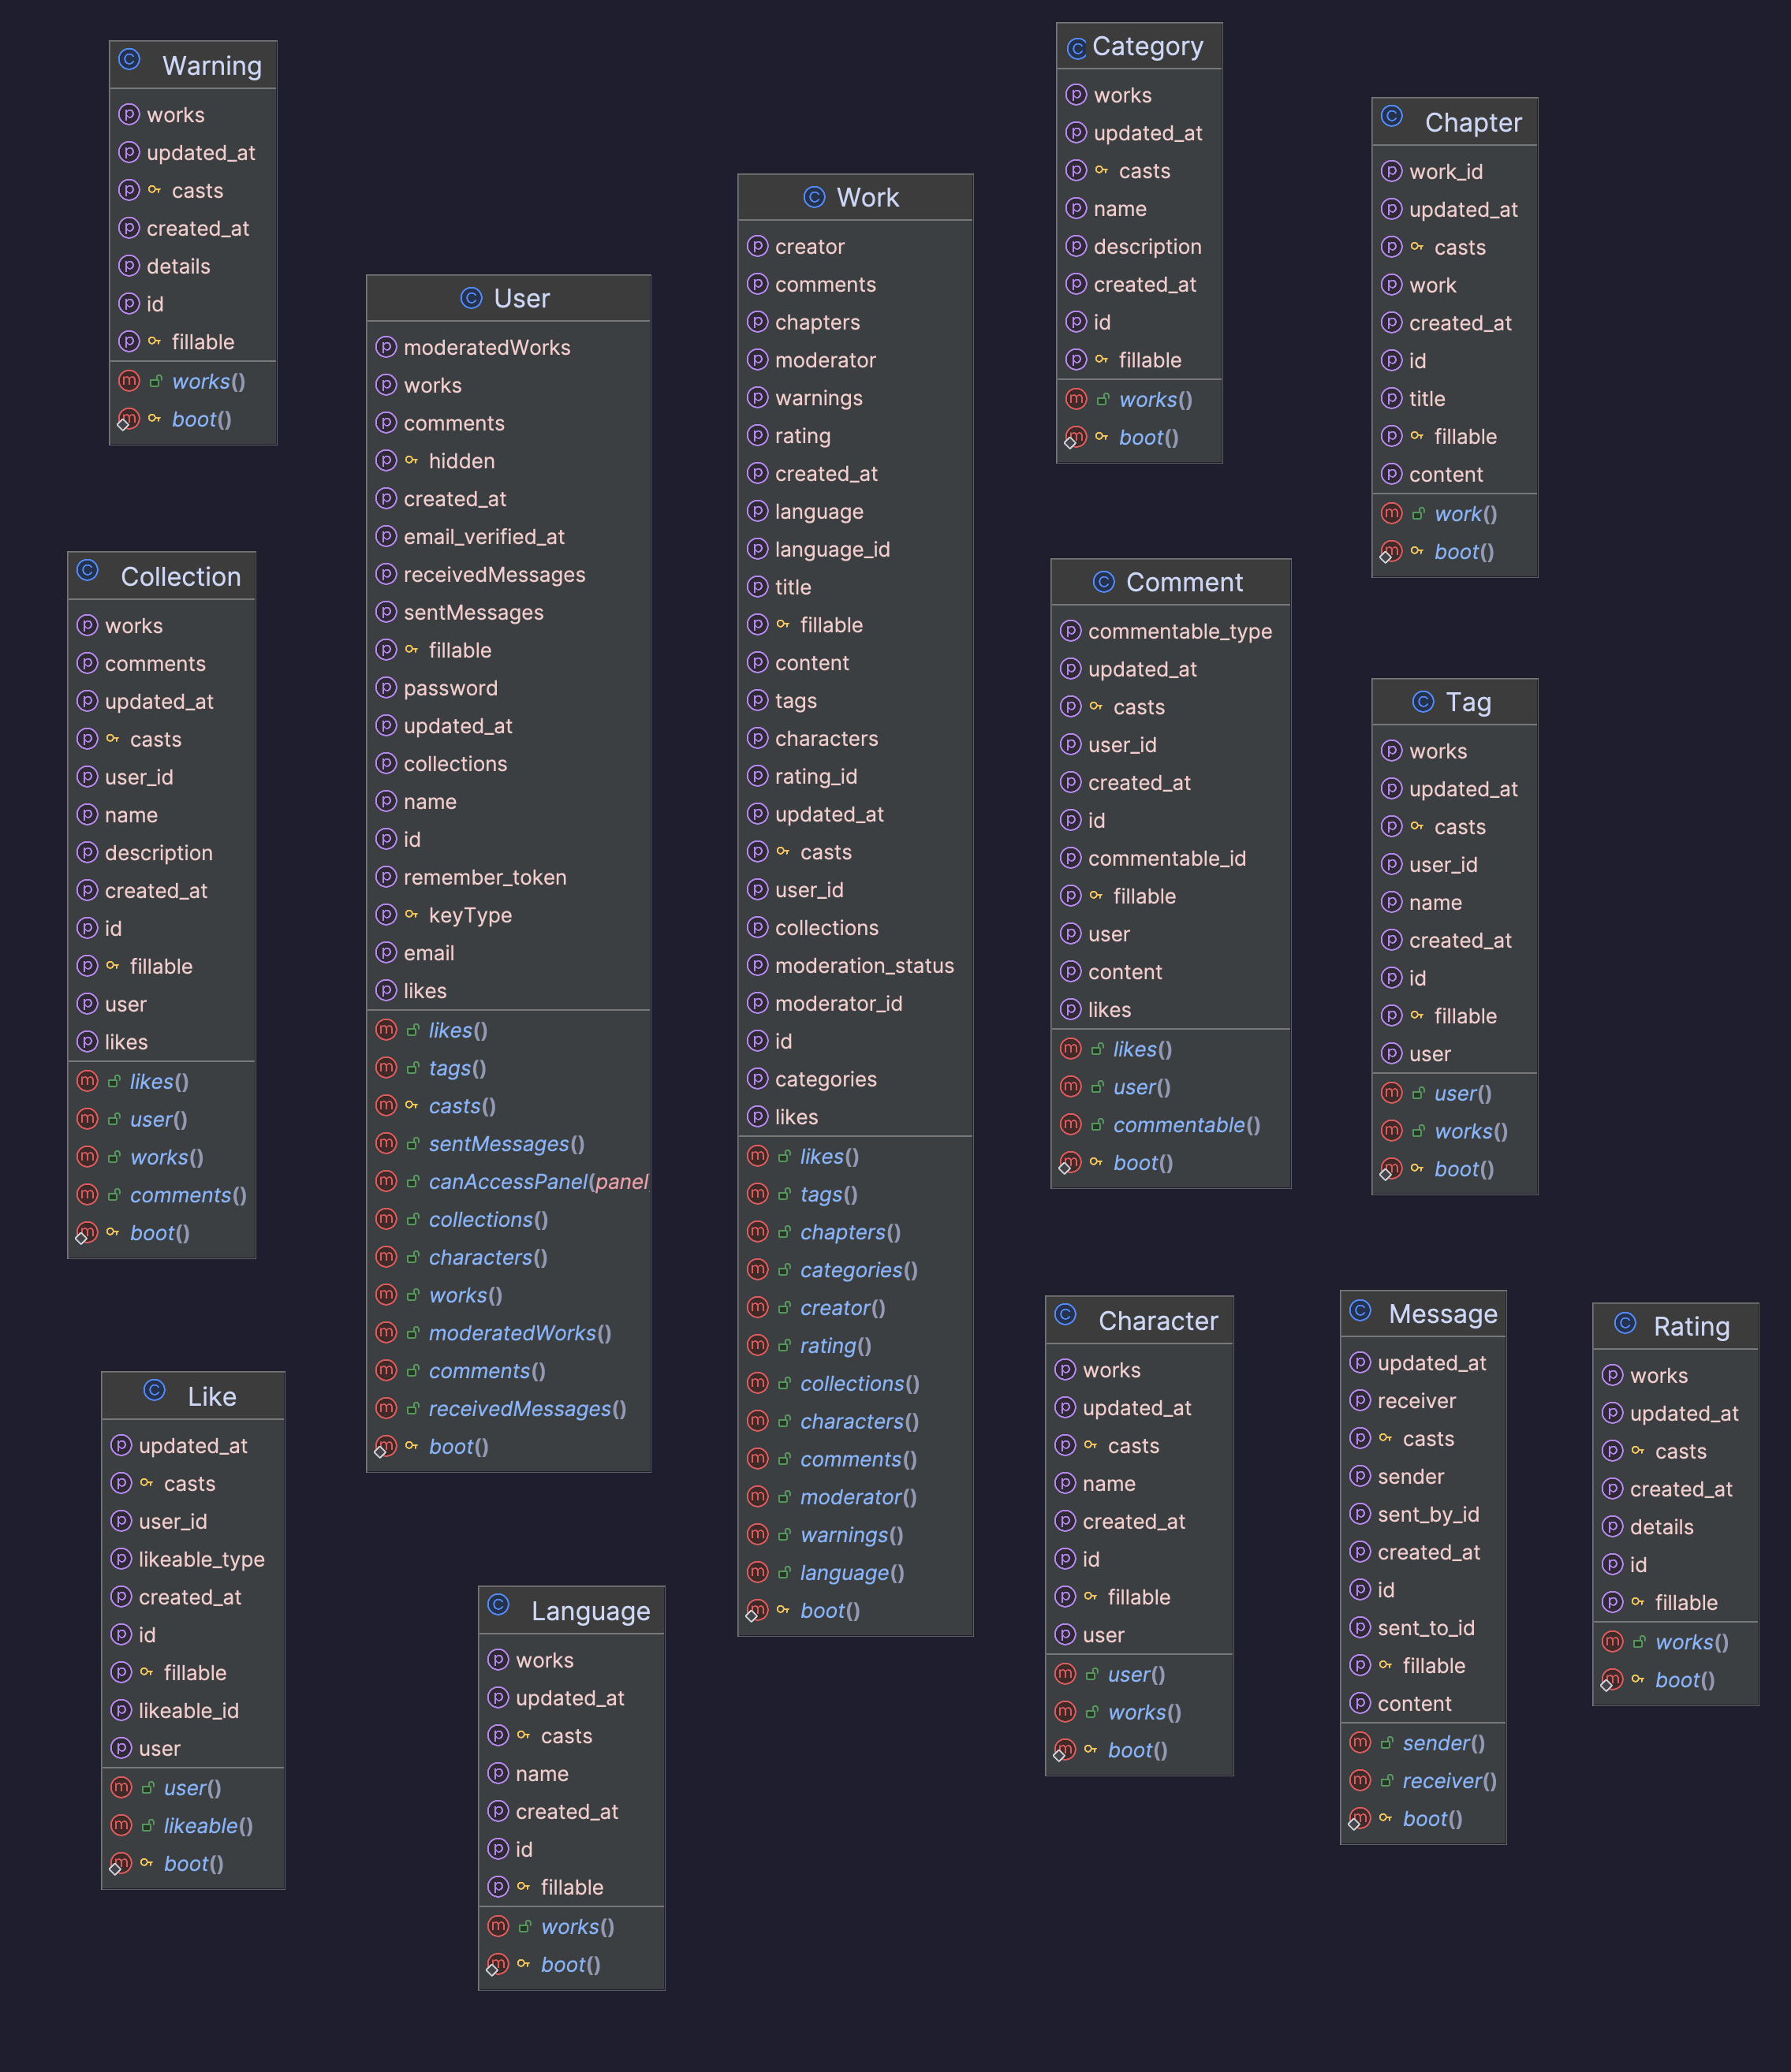
\includegraphics[scale=0.1]{./figures/models.png}
    \caption{Az alkalmazás modelljei}
    \label{fig:models}
\end{figure}


\textbf{Factory-k:}
A factory-k segítségével lehetőség van tesztadatok generálására az adatbázisba. A factory-k segítségével lehetőség van a modellekhez kapcsolódó adatok generálására, amelyeket a tesztelés során lehet használni. Ehhez a Laravel a Faker nevű könyvtárat használja, amely segítségével különböző típusú hamis, de struktúrális tekintetben helytálló adatokat lehet generálni.\\

\textbf{Seeder-ek:} A factory osztályok segítségével generált adatokat a seeder-ek segítségével lehet az adatbázisba betölteni, meghatározott mennyiségben és kapcsolatokkal. Külön jelentősége volt a \texttt{PermissionSeeder}-nek mely az alkalmazás jogosultságait definiálja.\\

\subsubsection{Üzleti logika réteg - BLL}


\textbf{Authentikáció:} Az authentikációra a Laravel Breeze \cite{LaravelBreeze} csomagot használtuk, mely egy minimális authentikációs rendszert biztosít. Az authentikációhoz szükséges routokat, controllereket, view-kat és middleware-eket a csomag automatikusan generálja. Az authentikációhoz szükséges adatbázis táblákat is a csomag generálja, így a felhasználók regisztrációja, bejelentkezése, jelszó visszaállítása, stb. egyszerűen megvalósítható.

A Breeze alapvetően Session alapú CSRF és CORS védelemmel rendelkező authentikációt biztosít a frontendek számára. Azonban maga a Breeze egy másik csomagra a Laravel Sanctum-ra \cite{LaravelSanctum} épít. Ennek előnye, hogy a Sanctum biztosít API Token alapú authentikációt is melyet a mobil kliens így ki tudott használni.\\

\textbf{Authorizáció:} Az authorizációra a Spatie cég által fejlesztett és karbantartott Laravel Permission csomagot \cite{LaravelPermissions} használtuk. A csomag segítségével lehetőség van jogosultságok (permissions) definiálására, azokhoz szerepkörök (roles) rendelésére, valamint a jogosultságok és szerepkörök alapján az authorizáció megvalósítására. A csomag a Laravel Policy-ket használja az authorizáció megvalósítására, amelyek segítségével a jogosultságokat és szerepköröket a modellekhez lehet rendelni.

Ennek előnye hogy ellenőrzéskor csak a jogosultság meglétét kell ellenőrizni, azonban a jogosultságok egységesen kioszthatók role-ok segítségével. Az alkalmazás 3 szerepkört valósít meg, melyek a \texttt{Registered}, \texttt{Moderator} és \texttt{Admin}. Az admin az alkalmazás ServiceProvider-ében minden ellenőrzésen automatikusan átengedésre kerül, így nem kell az össze jogosultságot hozzárendelni.\\

\subsubsection{Tesztelés}

Teszteltünk, PEST, mekkora fedettség, mi lett tesztelve és miért

\subsubsection{Admin felület}

Bár nem külön alkalmazás réteg de megemlítendő, hogy az admin felület megvalósítására a FilamentPHP csomagot \cite{FilamentPHP} használtuk a backend oldalon. Előnye, hogy a modell osztályokhoz definiálhatóak úgynevezett filament resource-ok melyek az admin felületen megjelenő mezőket és azok viselkedését definiálják. A csomag segítségével lehetőség van a modellek szerkesztésére, törlésére, listázására, stb. Az admin felület a \ref{fig:admin}. ábrán látható.

\begin{figure}[H]
    \centering
    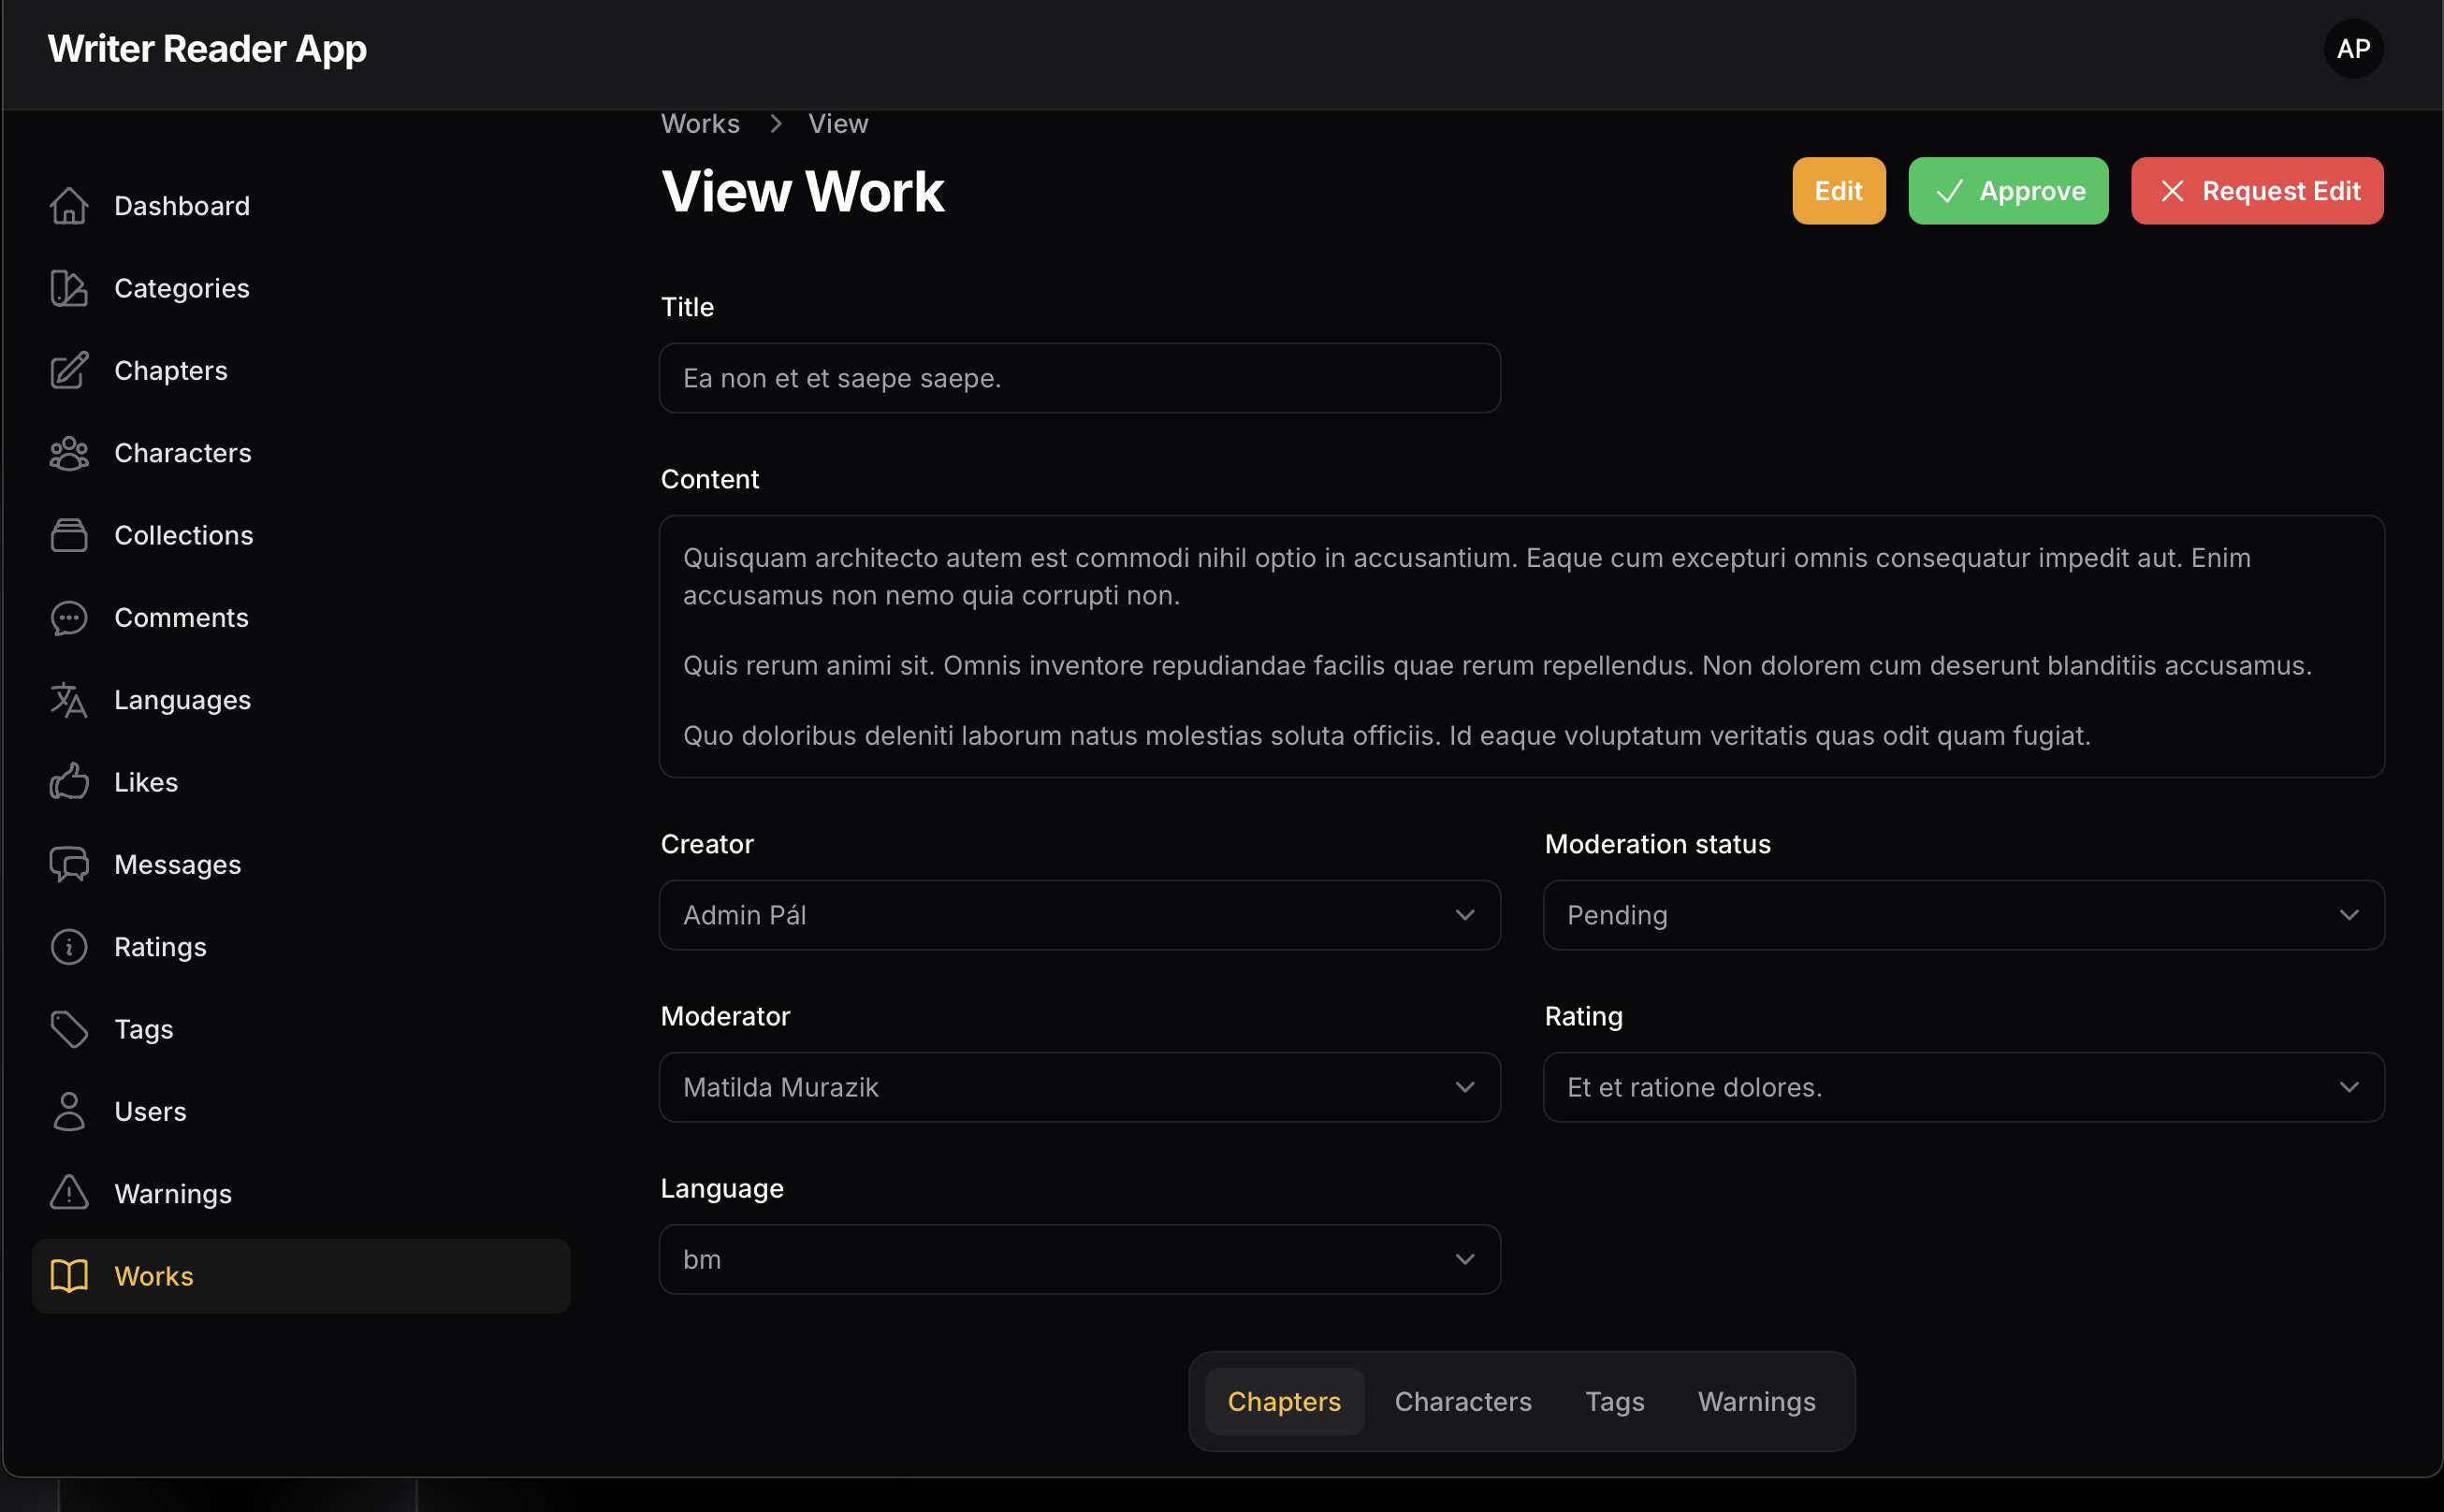
\includegraphics[scale=0.25]{./figures/admin-panel.png}
    \caption{FilamentPHP admin felület}
    \label{fig:admin}
\end{figure}

Az admin felülethez csak moderátor és admin jogosultságú felhasználó férhet hozzá. Azon belül az egyes modellek-hez való hozzáférést a policy osztályok szabályozzák de felülírható külön a filament resource-okon keresztül is.

Ezen kívűl az adminfelületen került megvalósításra a művek jóváhagyása is melyekre a moderátoroknak van jogosultságuk. A jóváhagyás után a művek publikussá válnak és megjelennek a felhasználók számára is, valamint automatikusan email értesítés küldődik a mű létrehozójának.
\subsection{Webes kliens megvalósítása}
Ez a fejezet a mobil kliens implementációjának részleteit mutatja be.
Nem minden funkció került megvalósításra, ezért csak azok a komponensek vannak részletezve amelyek a bemutatás során már működtek.

\subsubsection{Program felhasználói funkciói}
\begin{itemize}
    \item Regisztráció
    \item Bejelentkezés
    \item Kijelentkezés
    \item Oldalak közötti navigáció
    \item Művek, gyűjtemények böngészése, a kilistázó oldalon lapozás
    \item Művek, gyűjtemények megtekintése, fejezetek közötti és olvasása
    \item Művek megtekintése, fejezetek közötti és olvasása
    \item Bejelentkezett felhasználóknak további nézetek elérése
    \item Saját művek illetve gyűjtemények listájának megtekintése
\end{itemize}

\subsubsection{SPA Router}
A React applikációnkban a \texttt{React Router} (\url{https://reactrouter.com/}) \texttt{BrowserRouter}-e felelős az útvonalkezelésért.
Továbbá ez a csomag menedzseli a böngészési munkamenet (session) előzményeit és a ad számunkra navigációt elősegítő komponenseket (pl: Link, Navigate).
Az \texttt{SPA} (Single Page Application) azt jelenti, hogy csak egy webes dokumentumot tölt be a böngésző (ezesetben az \texttt{index.html}) és ennek a virtuális DOM-ját tölti fel dinamikusan.
Magukat az útvonalakat és a hozzá tartozó oldal-komponenseket a \texttt{AppRoutes} komponensünk definiálja.

\subsubsection{HTTP-kérések}
A HTTP kéréseket (GET, POST) a promise-alapú \texttt{Axios} (\url{https://axios-http.com/}) JavaScript könyvtárral intézzük.
A backenddel való kommunnikációhoz szükséges konfigurációk az \texttt{api/axios.jsx}-ben vannak

\subsubsection{Context Provider}
Az authentikáció után állapotaként a felhasználóhoz tartozó egyes adatokat (illetve az CSRF elleni tokent) a \texttt{ContextProvider} komponens szolgáltatja a struktúrában a gyerekeinek.
Azok az \texttt{useAuthContext} hook-ot használva tudnak hozzáférni az adatokhoz, megelőzve a sok props leadogatást a komponenseknek.

\subsubsection{Navigálás a weboldalon}
Navigálásban főként a felső sávban elhelyezkedő menük és gombok segítenek.
\begin{itemize}
    \item \textbf{/} (átirányít a /works-re)
    \item \textbf{/works}
    \item \textbf{/collections}
    \item \textbf{/reader}
    \begin{itemize}
        \item \textbf{\dots/[workID]}
    \end{itemize}
    \item \textbf{/collection}
    \begin{itemize}
        \item \textbf{\dots/[collectionID]}
    \end{itemize}
    \item \textbf{/login} (visszairányít, ha a felhasználó már be van jelentkezve)
    \item \textbf{/register} (visszairányít, ha a felhasználó már be van jelentkezve)
    \item \textbf{/profile} (átirányít a /login-ra, ha a felhasználó nincs bejelentkezve)
    \item /\textbf{account} (átirányít a /login-ra, ha a felhasználó nincs bejelentkezve)
    \item \textbf{/editor} (mű szerkesztő, még nem kommunikál)
\end{itemize}

\subsubsection{Webes felhasználói felület}
A weboldal felülete a \texttt{React MUI} (félkész és konfigurálható) komponenseivel van felépítve.
Ez a csomag azért lett választva, hogy a dizájn a mobilossal valamilyen szinten megegyezzen.
Ahogyan már az előbbiekben említettük, a SPA egyetlen dokumentumát tölti fel az alkalmazás;
emiatt a navigáció zökkenésmentesnek hat.

A weboldal látogatásakor tipikusan a Művek böngészése oldalra kerül a felhasználó.

\begin{figure}[H]
    \centering
    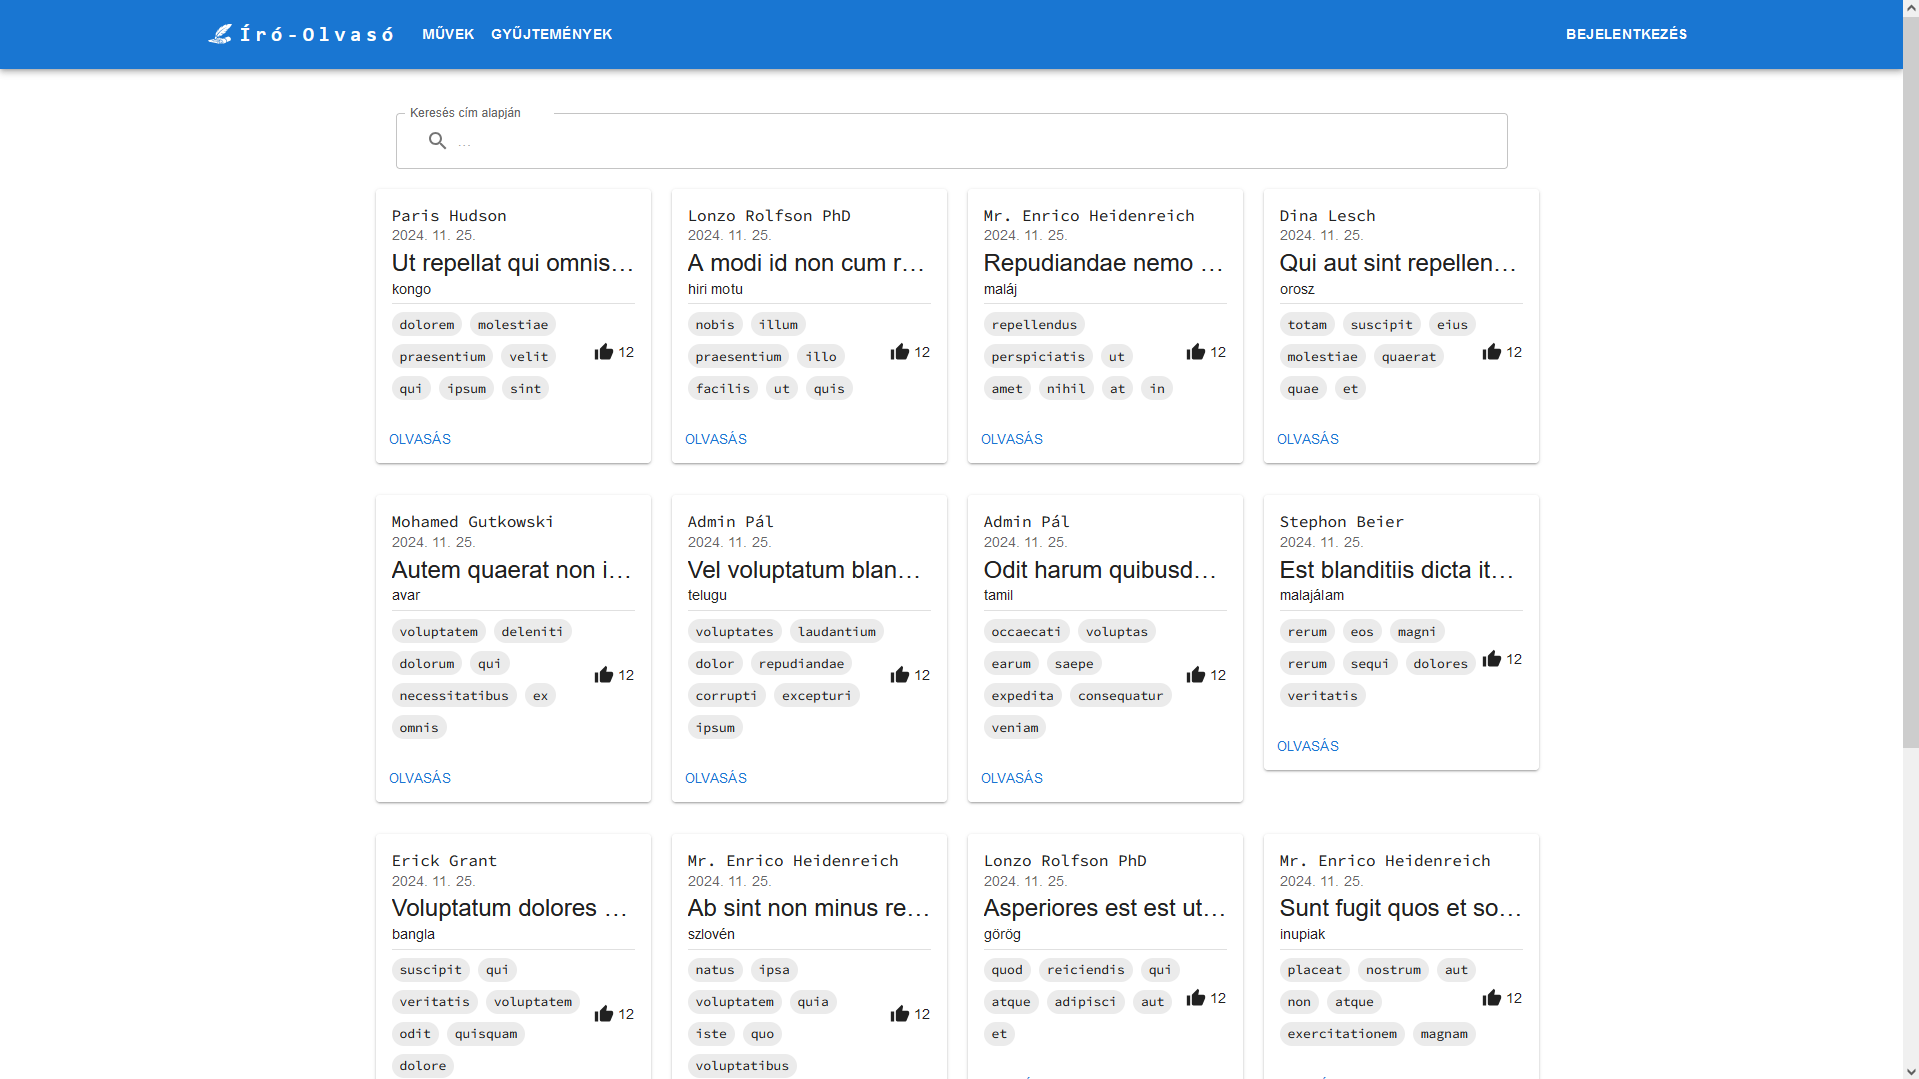
\includegraphics[scale=0.3]{./figures/works-page.png}
    \caption{/works Művek oldal}
    \label{fig:works-page}
\end{figure}

A felső navigációs sávban láthatja a másik nem bejelentkezett látogatók
számára is elérhető Gyűjtemények oldalt, továbbá a Bejelentkezés gombot.
Kisebb képernyőmérettel vagy ablakmérettel az oldal tartalma is alkalmazkodik.
Ilyenkor a navigációs sáv opció egy lenyíló menüben érhetők el.

\begin{figure}[H]
    \centering
    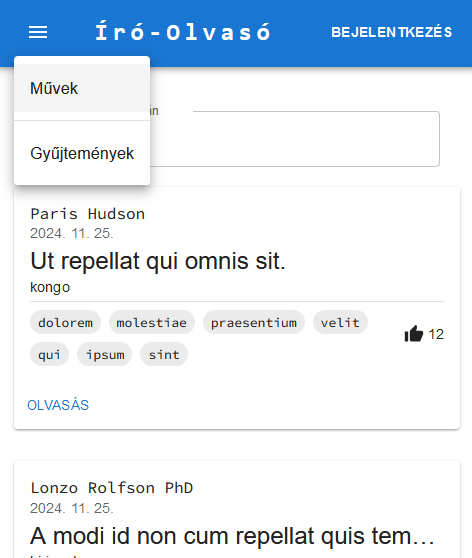
\includegraphics[scale=0.5]{./figures/navbar-small.png}
    \caption{Művek oldal kisebb méretben}
    \label{fig:navbar-small}
\end{figure}

Az oldal legalján lehet lapozni, mivel nem minden kártya fér ki egy oldalra (jelenleg 15 kártya / oldal van beállítva).
A szélső gombok sorrendben az első és utolsó oldalra lapoznak. A Gyűjtemények oldal hasonló kártyákkal és lapozással van ellátva.

\begin{figure}[H]
    \centering
    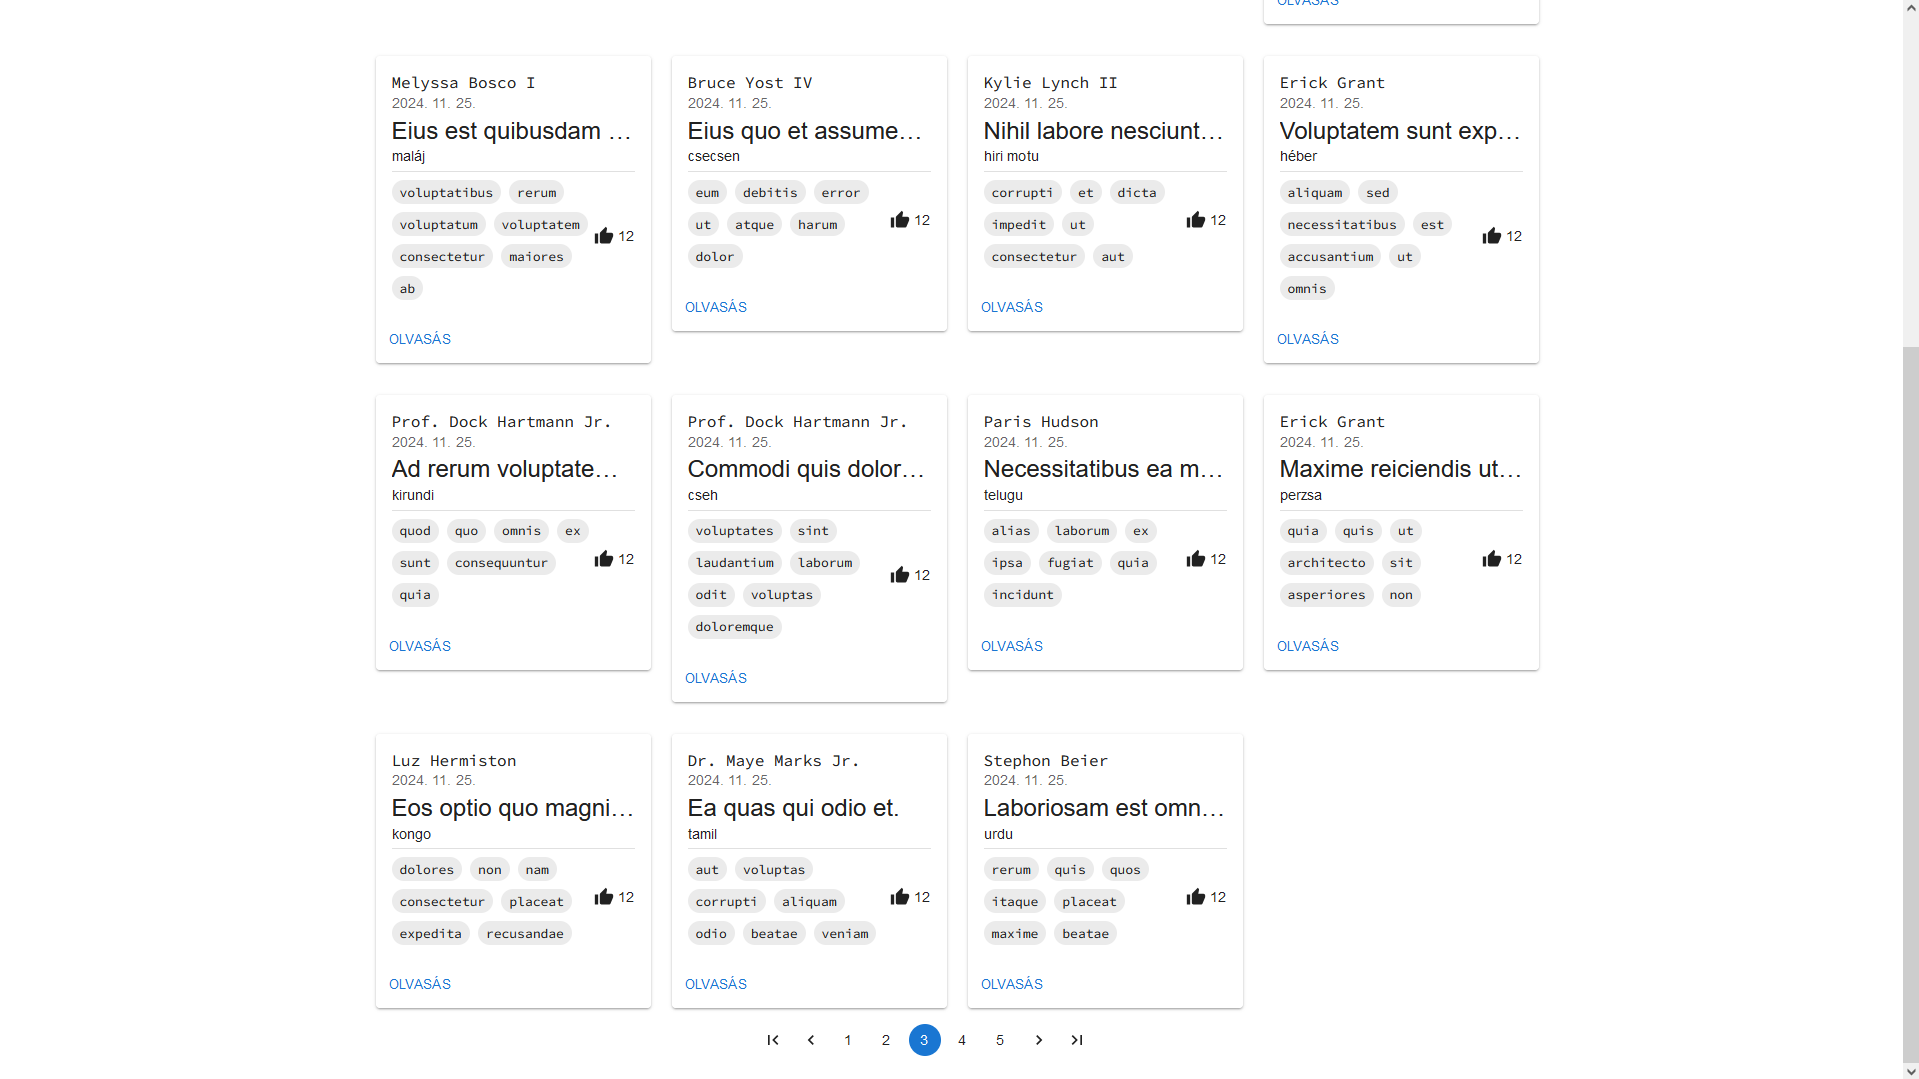
\includegraphics[scale=0.3]{./figures/works-pagination.png}
    \caption{Művek oldal lapozása}
    \label{fig:works-pagination}
\end{figure}

Ha egy Gyűjteményt a kártyáján megjelenő gombbal megnyitunk, átvisz minket a /collection/[ID] útvonalra.
Itt a gyűjteménybe szedett művek listáját kapjuk meg, továbbá láthatjuk, hogy mennyi kedvelést illetve milyen hozzászólásokat kapott.

\begin{figure}[H]
    \centering
    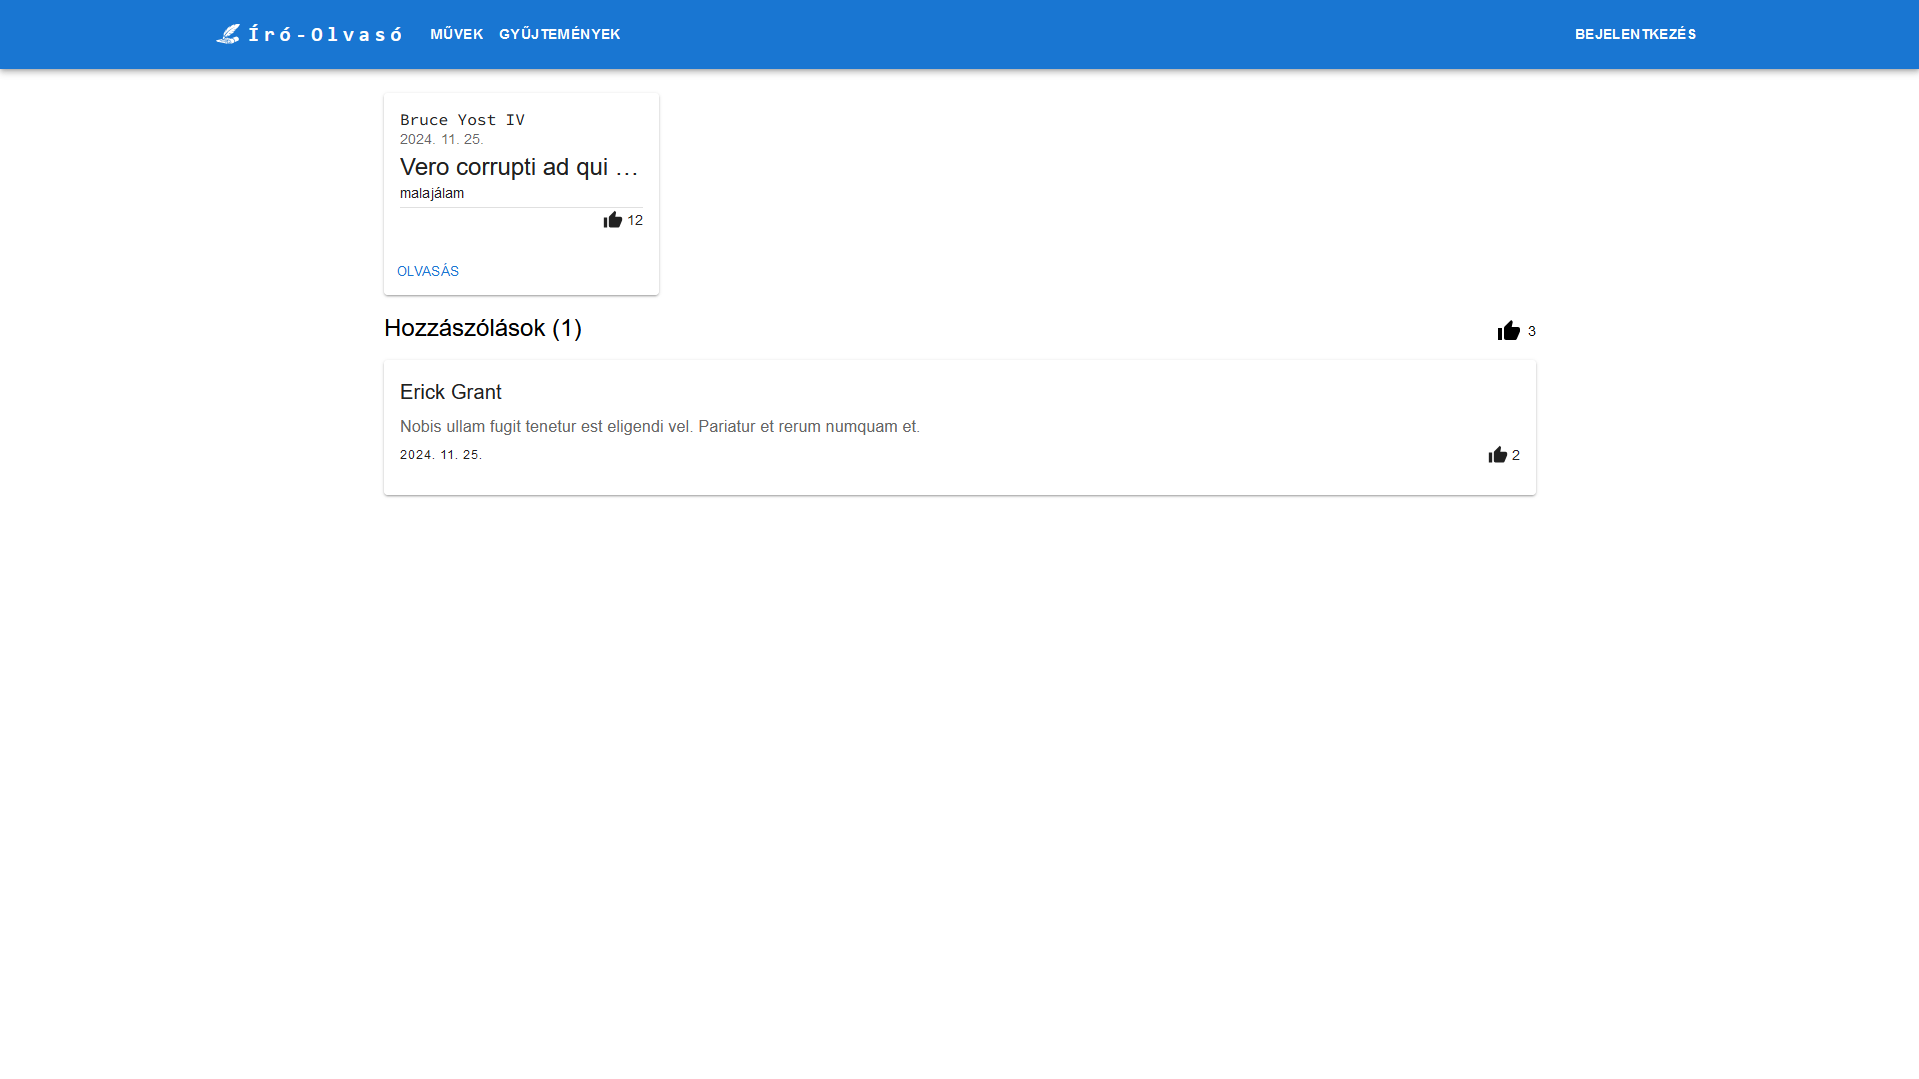
\includegraphics[scale=0.3]{./figures/collection-page.png}
    \caption{Gyűjtemény megtekintése}
    \label{fig:collection-page}
\end{figure}

A gyűjteményben lévő műveket is meg lehet nyitni, hogy elolvassuk.




\subsection{Mobil kliens megvaklósítása}
Ebben a fejezetben a mobil kliens implementációjának részleteit mutatjuk be. Sajnos előre nem látható és
technikai nehézségek miatt a megszabott határidőig nem sikerült a specifikációban előírt minden funkciót elkészíteni, 
itt csak a működő komponensek kerülnek bemutatásra.

A programban a következő főbb funkciók érhetők el: 
\begin{itemize}
    \item Regisztráció
    \item Bejelentkezés
    \item Művek böngészése
    \item Művek részleteinek megtekintése
    \item Művek olvasása
    \item Kedvelés küldése
    \item Hozzászólás írása
    \item korábbi privát üzenetek megtekintése
\end{itemize}

A mobilé architektúrája rétegekre bontható, ezek kifejtésében bemutatjuk nagyvonalakban a kód felépítését és a használt technológiákat.
 a használt androidos technológiákat.


\subsubsection{Adatlekérdezés (HTTP kliens)}
A mobil kliens a szerverrel való hálózati kommunikációt a Retrofit könyvtár segítségével valósítja meg.
A Retrofit egy nyílt forráskódú Android és Java HTTP-kliens, amely a REST API-k hívását teszi lehetővé.


\paragraph{REST API interfész}
Az API-hívások kezelésére a \texttt{WriterReaderApi} interfész definiálja a szerver által támogatott végpontokat. 
Az egyes metódusok Retrofit-es annotációkkal vannak ellátva, amelyek a megfelelő HTTP metódusokat és a végpontokat definiálják.
Az interfész nem tartalmazza az összes szerver által biztosított végpontot, hanem csak amelyek a mobil klens eddigi 
funkcióihoz szükségesek:

\begin{itemize}
    \item \textbf{Művek kezelése:}
    \begin{itemize}
        \item \texttt{getWorks}: Az összes mű lekérdezése.
        \item \texttt{getWork}: Egy adott mű részleteinek lekérdezése azonosító alapján.
    \end{itemize}
    \item \textbf{Felhasználók kezelése:}
    \begin{itemize}
        \item \texttt{getUsers}: Az elérhető felhasználók listázása.
        \item \texttt{getUser}: Egy adott felhasználó adatainak lekérdezése azonosító alapján.
        \item \texttt{getCurrentUser}: Az aktuálisan bejelentkezett felhasználó adatainak lekérdezése token alapján.
    \end{itemize}
    \item \textbf{Hozzászólások és kedvelések kezelése:}
    \begin{itemize}
        \item \texttt{postComment}: Hozzászólás küldése.
        \item \texttt{postLike}: Kedvelés hozzáadása.
        \item \texttt{deleteLike}: Kedvelés törlése.
    \end{itemize}
    \item \textbf{Hitelesítés:}
    \begin{itemize}
        \item \texttt{register}: Új felhasználó regisztrációja.
        \item \texttt{login}: Bejelentkezés a rendszerbe.
        \item \texttt{logout}: Kijelentkezés az aktuális munkamenetből.
    \end{itemize}
\end{itemize}

A HTTP kommunikációban JSON objektumokat használunk, melyeket kotlin osztályokra képződnek le
A JSON objektumok és Kotlin osztályok közti átalakítást a \textbf{Moshi} könyvtár segítségével végezzük el. 

\paragraph{Retrofit konfiguráció}
A REST API végpontok eléréséhez egy Retrofit klienst kell létrehozni, itt konfiguráljuk például az időtúllépési értékeket, a moshi JSON adaptert
és az alap URL-t a szerverhez, ami jelenleg \texttt{http://10.0.2.2}, ez egy alias és az android emulátoron a host gép címét jelenti.
A retrofit kliens a \texttt{WriterReaderApplication} osztályban az alkalmazáés indulásakor jön létre.

\subsubsection{Adatelérés (Repository)}

Az alkalmazás az adatelérésre egy a hálózati kommunikáció feletti absztrakciós réteget használ (\textbf{data access layer}), 
ami lényegeében egy \texttt{ApiMAnager} nevű wrapper osztály a Retrofit kliens és a hálózati hívások köré. Megkönnyíti a magasabb szintű kódból való használatot.
AZ adatelérési réteg két fontosabb feladata az API-hívások kezelése és a hibakezelés.
Az osztáy suspend fun metóduasi gondoskodnak arról,
hogy a hálózati hívások csak corutineokon belül történjenek, így ne blokkolják a UI szálat,
\paragraph{Hibakezelés} A válaszok kezeléséhez a \texttt{Retrofit Response} osztályt használja, 
amely tartalmazza a HTTP státuszkódot és a szerver által küldött adatokat. 
Minden API-hívás esetén figyelembe vesszük a lehetséges hibákat, mint például hálózati időtúllépést vagy nem várt szerverhibákat, 
hogy megfelelő visszajelzést adhassunk a felhasználónak. Az \texttt{ApiMAnager} metódusai onSuccess és onError callback 
függvényeket várnak paraméterként, amelyek a hálózati hívások végrehajtásakor hívódnak meg.

Az \texttt{ApiMAnager} osztályt az alkalmazás indulásakor pédányosítjuk így az egész alkalmazásban elérhető lesz.


\subsubsection{UI réteg (UI Layer)}

A alkalmazás egyes képernyőit MVI (Model-View-Intent) architektúra szerint valósítottuk meg.
Ennek az architektúrának 4 komponense van
\begin{itemize}
    \item \textbf{Model} 
    \item \textbf{Intent} 
    \item \textbf{View} 
    \item \textbf{View-Model}
\end{itemize}

\paragraph{Model}
A Model az alkalmazás állapotának (State) egy reprezentációja. Ez a komponens tartalmazza a képernyőhöz 
szükséges összes adatot és a felhasználói interakciók eredményét. 
Az állapot megváltozása új state objektum létrehozásával történik.

\paragraph{Intent}
Az Intent-ek képviselik a felhasználói interakciókat és a képernyő eseményeit (például: egy gomb lenyomása). 
Az Intent-ek explicit módon jelzik a ViewModel-nek, hogy milyen műveleteket kell végrehajtania.

\paragraph{View}
A View a Jetpack Compose deklaratív UI komponensei által megvalósított felhasználói felület.
Az composable elemek kizárólag a State alapján frissülnek.
A View nem tartalmaz logikát, hanem kizárólag az állapot megjelenítéséért felelős.


\paragraph{View-Model}
A ViewModel felel az Intent-ek feldolgozásáért és az állapot frissítéséért. 
Ez a komponens biztosítja a State folytonosságát és kezeli az üzleti logikát,
például hálózati kérések indítását.
A ViewModel figyeli az Intent-eket, végrehajtja a szükséges műveleteket, és az új állapotot a View felé közvetíti.




\section{Telepítési lerírás}
\label{sec:installation}
\section{A program készítése során felhasznált eszközök}
\label{sec:softwares}

\subsection{Backend szoftverek}

\begin{itemize}
    \item Laravel 11, PHP 8.2, Composer
    \item Package-k: 
    \begin{itemize}
        \item FilamentPHP: admin felület,
        \item Laravel-Permissions: jogosultság kezelés,
        \item Laravel Breeze: authentikáció,
        \item Laravel Sail: Docker konténerek kezelése
        \item Pest: PHP tesztelés
    \end{itemize}
    \item Docker (Desktop): konténerizáció
    \item MySQL: adatbázis (konténerizálva)
    \item MailPit: mail küldés tesztelése (konténerizálva)
    \item PhpStorm IDE: fejlesztői környezet
\end{itemize}

\subsection{Webes szoftverek}

\begin{itemize}
    \item Vite 5.4 + React 18.3 (JSX)
    \item npm: JavaScript csomagkezelő
    \item Package-k: 
    \begin{itemize}
        \item React Router: navigáció
        \item MUI, Emotion, Roboto: UI React komponensek
        \item Axios: kérések
        \item js-cookie: sütik kezelése
        \item mui-markdown: markdown megjelenítése
        \item react-md-editor: markdown szerkesztő
        \item ESLint: kód analízis
    \end{itemize}
    \item Firefox, Chrome, MS Edge: böngészők
    \item Visual Studio Code: fejlesztői környezet
\end{itemize}
\section{Összefoglalás}
\label{sec:summary}

A projektmunka során specifikáltuk, megterveztük, és implementáltuk a Közösségi Író-olvasó oldalt. Az alkalmazás célja, hogy egy olyan platformot biztosítson, ahol az írók megoszthatják műveiket, és az olvasók könnyen megtalálhatják az érdeklődésüknek megfelelő tartalmakat. Az alkalmazás lehetőséget ad az írók számára, hogy műveiket kategóriákba sorolják, és a felhasználók számára, hogy kedvenc műveiket kedvelhessék és kommentekkel láthassák el.

Az alkalmazás kliens-szerver architektúrát használ, lazán csatolt módon Rest API-kon keresztül kommunikálnak a kliensek a szerverrel. A backend a Laravel nevű PHP keretrendszert használva készült el. Az alkalmazás kliens oldali része egy webes frontend és egy mobil kliens. A webes frontend a React keretrendszerre épül, a mobil kliens pedig a JetPack Compose keretrendszer segítségével készült. 

Munkánkat alapos tervezéssel, és architektúrális döntések meghozásával támogattuk, mint például a különböző felhasznált technológiák és keretrendszerek kiválasztása és alkalmazása. Jelentős mennyiségű implementációs munkát végeztünk, és bár minden specifikált funkció nincs még implementálva, az elkészült alkalmazás már használható és stabil, biztonságos és könnyen bővíthető alapot nyújt jövőbeli fejlesztésekhez.
\section{Továbbfejlesztési lehetőségek}
\label{sec:improvements}

%--------------------------------------------------------------------------------------
% Bibliográfia [Bibliography] - Ha üres kommenteld ki [Uncomment if empty]
%--------------------------------------------------------------------------------------

\newpage
\thispagestyle{empty}
\pagenumbering{gobble}
{
    \footnotesize  % Kisebb betűméret [Smaller font size]
    \bibliographystyle{plain}
    \bibliography{mybib}
}
\addcontentsline{toc}{section}{Hivatkozások}

\end{document}